\chapter{Utilities}

%\section{Input File GUI} 
%\label{sec:GUI}
%This script provides a graphical user interface (GUI) with which the user 
%may create input files for use in simulations.  The GUI is written 
%in Python and uses the wxWidgets for Python module, which may be found at
%http://wxpython.org/download.php. The GUI was written using 
%Python 2.7.6 and wxPython 3.0.1.1.
%
%Upon installing the wxPython bundle compatible with your version of 
%Python, the GUI may be launched by opening
%the terminal, navigating to the /Scripts/Input\_File\_Generation/
%which contains the GUI script, and executing the following command:  \\ \\
%%
%\texttt{> python InputFileGUI\_v1\_2.py}
%%
%
%The GUI will launch to display the screen shown in Figure \ref{fig:GUIscreenshot}
%
%\begin{figure}[h]
% \centering
% 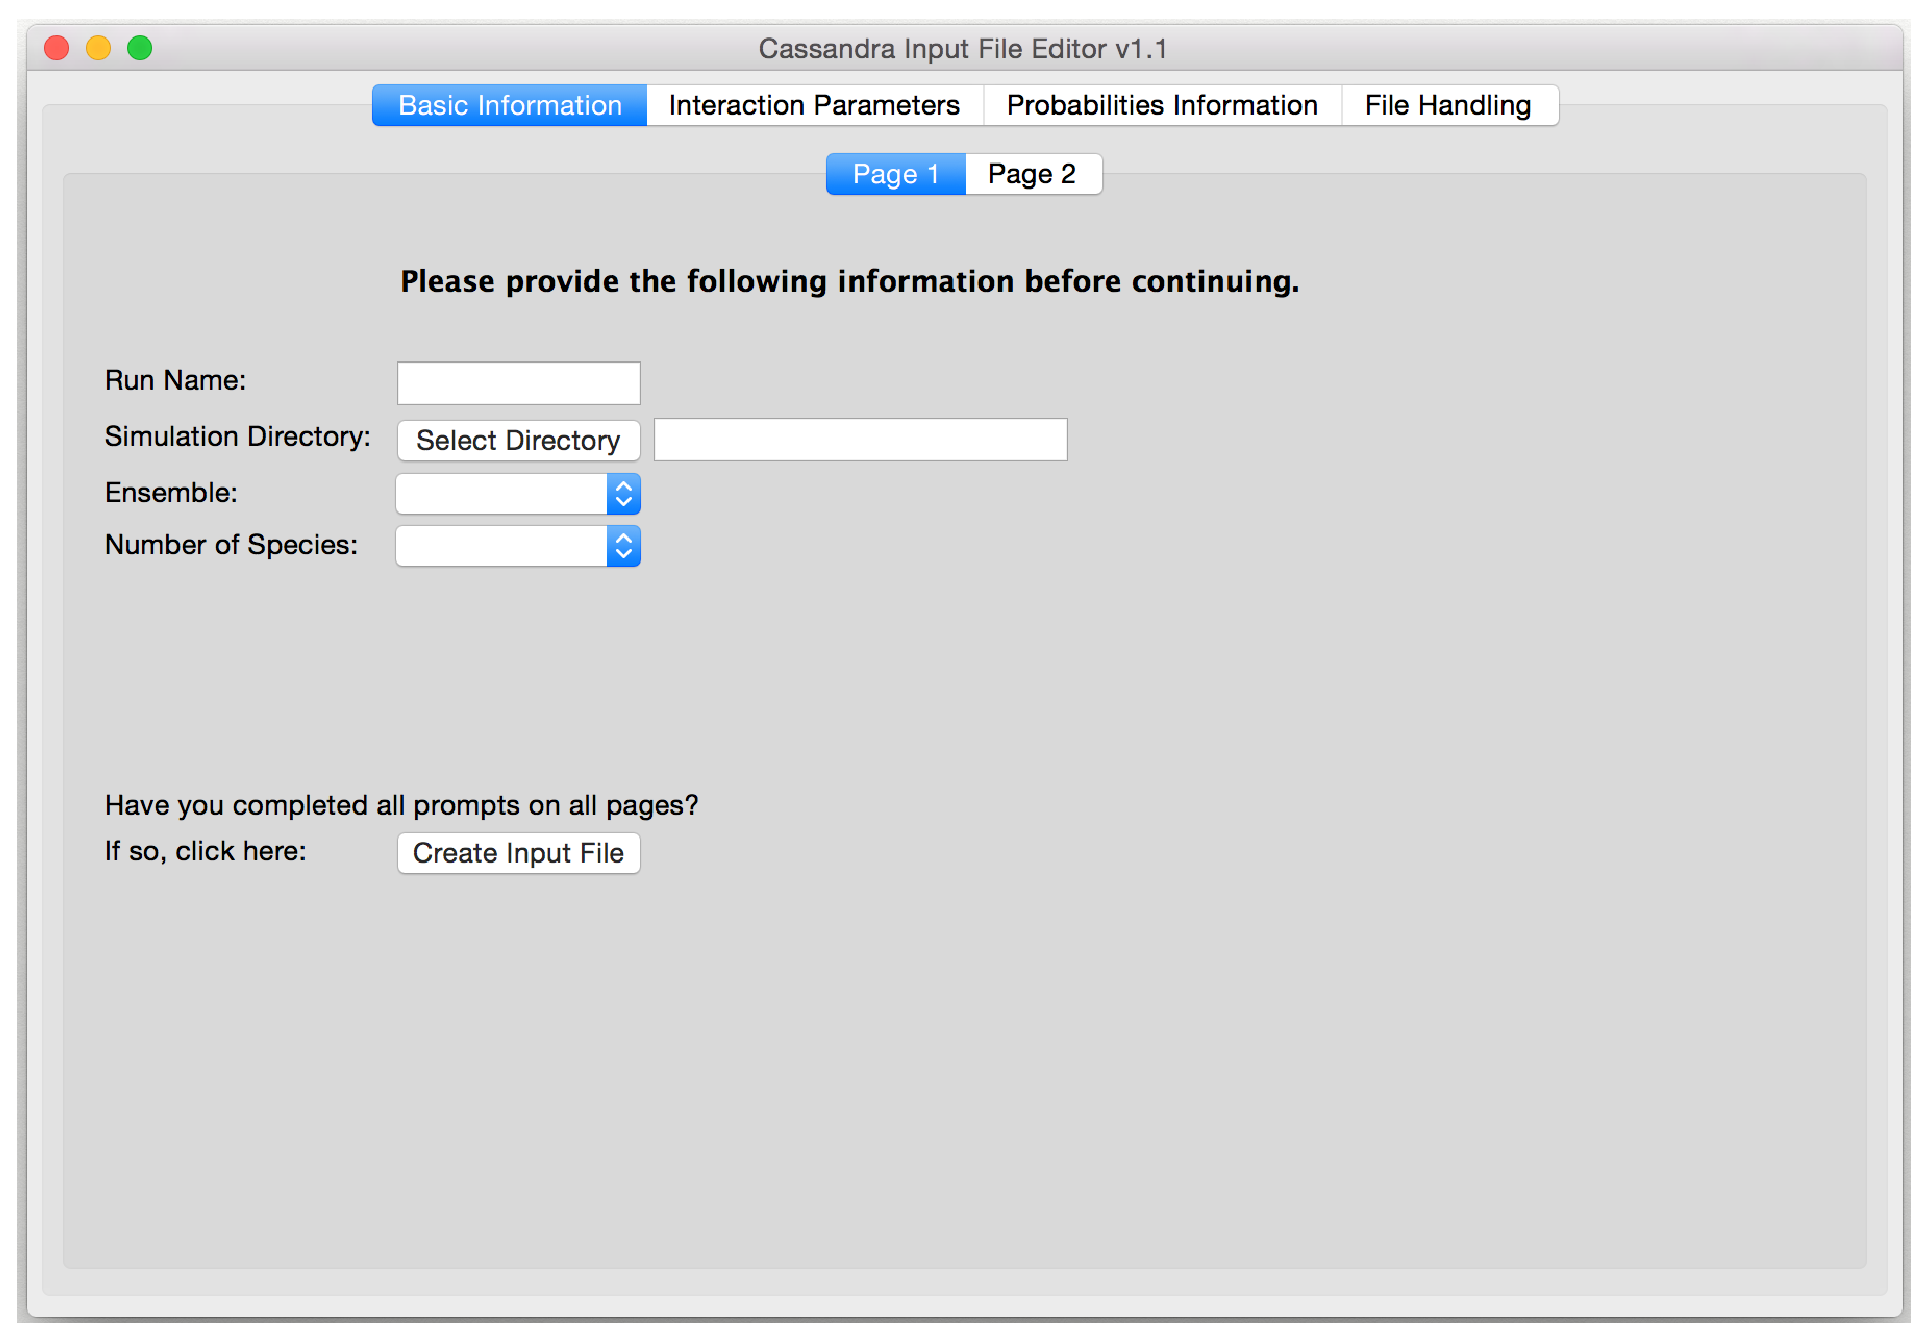
\includegraphics[width=\textwidth]{GUI_screenshot.eps}
% \caption{Cassandra Input File Graphical User Interface}
% \label{fig:GUIscreenshot}
%\end{figure}
%
%Complete all prompts as instructed on all panels of the GUI. 
%Once all information has been provided, return to the Basic Information-Page 1 
%section and click on ``Create Input File'' to create the input file. Note that if no 
%value is entered for a required prompt, the GUI will inform the user 
%via a KeyError message in the terminal.
%
%If a given parameter is to be input at a later point in time, 
%enter ``?'' and subsequently use a text editor to enter the 
%desired value in the input file manually.  
%
%If creating multiple input files, it is strongly encouraged to exit the GUI
%and restart from the terminal each time a file is created, otherwise, data from the 
%previous file may leak to the next file.
%
%A set of executable files are provided that do not require the installation
%of the wxPython module. These executables are available for Unix-like systems.
%In order to run these, the user must change the access permissions of the executable through the
%command \\ \\
%
%\texttt{> chmod +x InputFileGUI\_v1\_2\_UNIX.exe}. 
%
%Then, the user can execute the GUI by typing \\ \\
%\texttt{> ./InputFileGUI\_v1\_2\_UNIX.exe}. 

\section{Generate a Molecular Connectivity File}
\label{sec:mcfgen}

The script \texttt{mcf\_gen.py} is a tool that aims to ease the setup of molecular connectivity files from scratch (see section \ref{sec:MCF_File} to learn more
about MCFs), as the generation of these files by hand can be error prone. 
In this section, a pentane MCF will be generated to demonstrate the use of this tool.
The Transferable Potentials for Phase Equilibria (TraPPE) force field will be used to represent the pentane molecular interactions. 
This force field involves a pairwise-additive 12-6 Lennard-Jones potential to represent the dispersion-repulsion interactions. Additionally, bond angles and dihedral angles are represented through
harmonic and OPLS functional forms, respectively. Bond lengths are kept constant. The force field mathematical
expression becomes

\begin{align*}
U = \sum_{angles} K_\theta(\theta-\theta_0)^2 +
\sum_{dihedrals} \frac{1}{2}K_1[1+cos(\phi)]+\frac{1}{2}K_2[1-cos(2\phi)] + \frac{1}{2}K_3[1+cos(3\phi)]+\frac{1}{2}K_4[1-cos(4\phi)] + \\
\sum_{i} \sum_{i>j} 4 \epsilon_{ij} \left [  \left ( \frac {\sigma_{ij}} { r_{ij} }\right )^{12} - \left ( \frac {\sigma_{ij}} { r_{ij} }\right )^{6}\ \right ]
\end{align*}

First, generate (or obtain) a PDB file or a CML file. To generate a PDB or CML file, 
software such as Gaussview or Avogadro can be used. Alternatively, PDB files can
be downloaded from the internet (e.g. www.rcsb.org). In this example, a pentane PDB file using the 
program Gaussview v5.08 was be generated, as shown below. \\

%After launching the Gaussview interface, click on the ``Element Fragment'' button located on the upper-left corner of the
%window.
%
%
%\begin{figure}[h]
%\begin{center}
%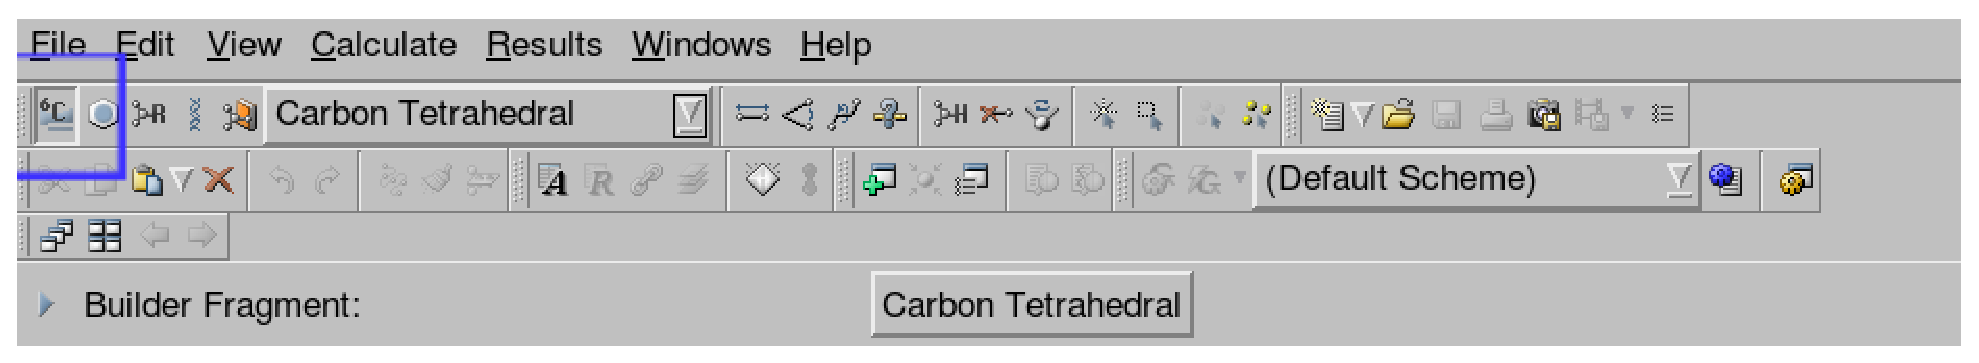
\includegraphics[height=1in]{gaussian1final.eps}
%\end{center}
%\end{figure}
%
%A periodic table will appear. Click on the ``Carbon'' button. 
%
%\begin{figure}[h]
%\begin{center}
%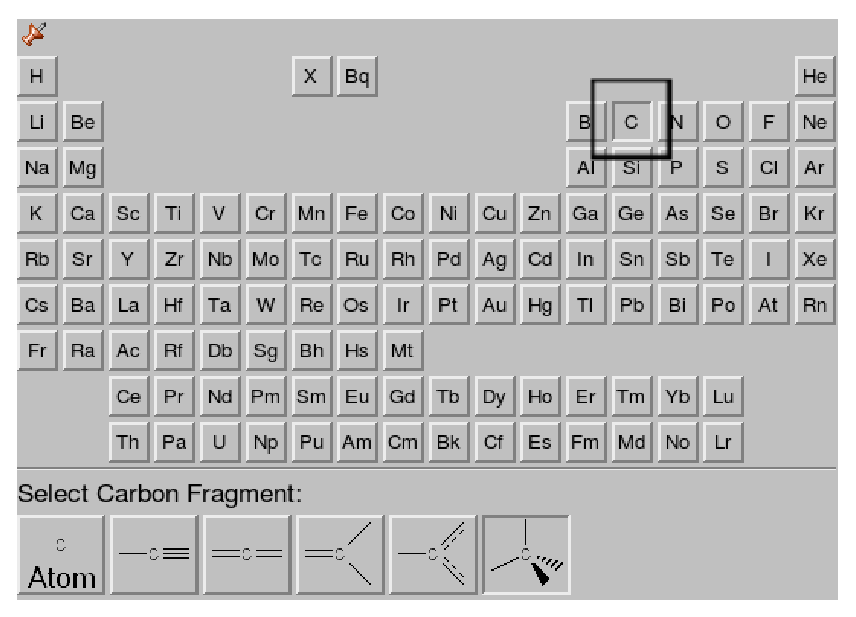
\includegraphics[height=3in]{gaussian2final.eps}
%\end{center}
%\end{figure}
%
%Click on the main workplace to insert the first $CH_4$ fragment.
%To increase the chain length, click on a hydrogen attached to the carbon. 
%
%\begin{figure}[h]
%\begin{center}
%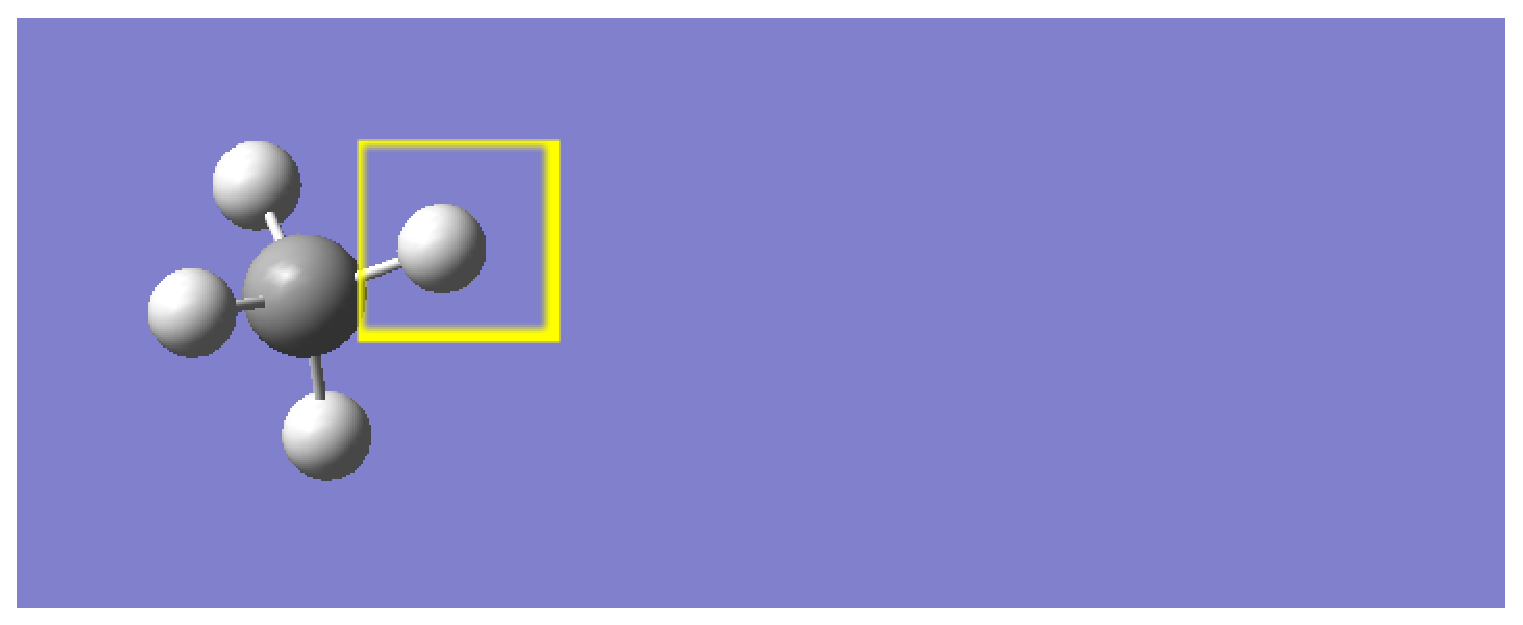
\includegraphics[height=2in]{gaussian3final.eps}
%\end{center}
%\end{figure}
%
%The final pentane structure should look something like this
%
%\begin{figure}[h]
%\begin{center}
%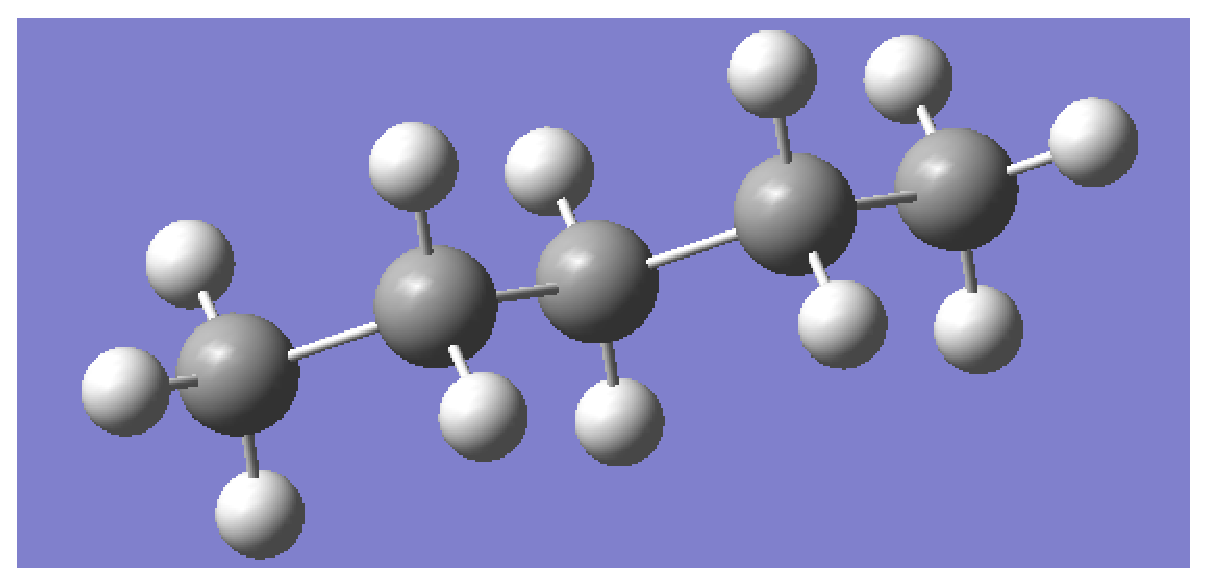
\includegraphics[height=2in]{gaussian4final.eps}
%\end{center}
%\end{figure}
%\vspace{3in}
%Right click on any place of the workplace, select the option builder and then
%select delete atoms.
%
%\begin{figure}[h]
%\begin{center}
%\includegraphics[height=2.5in]{gaussian5final.eps}
%\end{center}
%\end{figure}
%
%Click on all the hydrogen atoms to delete them 
%
%\begin{figure}[h]
%\begin{center}
%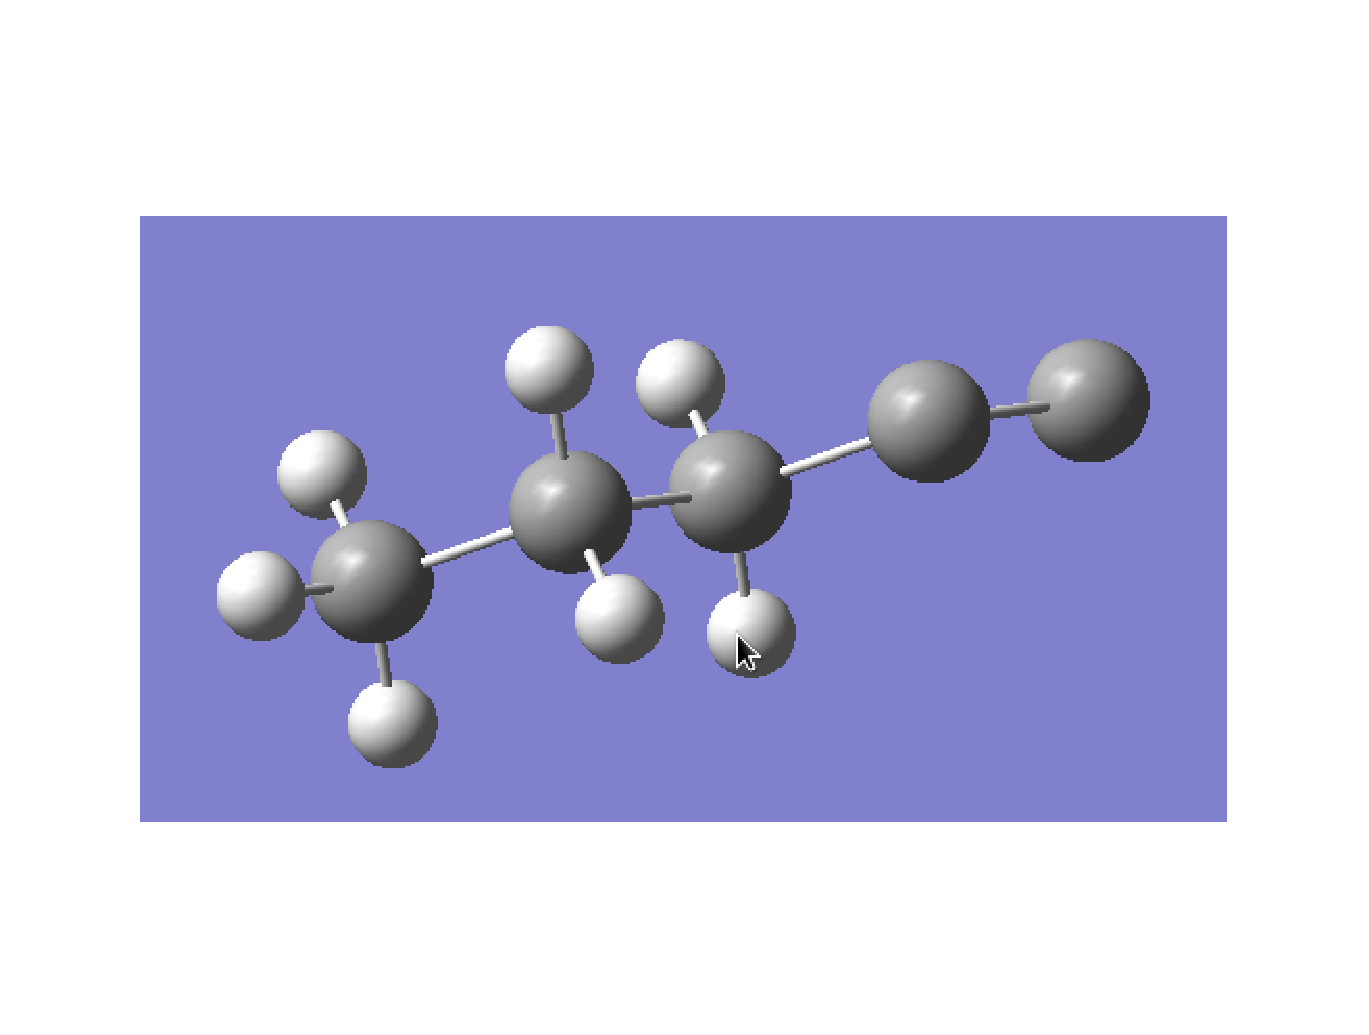
\includegraphics[height=2.5in]{gaussian7final.eps}
%\end{center}
%\end{figure}
%
%\vspace{3in}
%Go back to main menu, click on File - Save.
%
%\begin{figure}[h]
%\begin{center}
%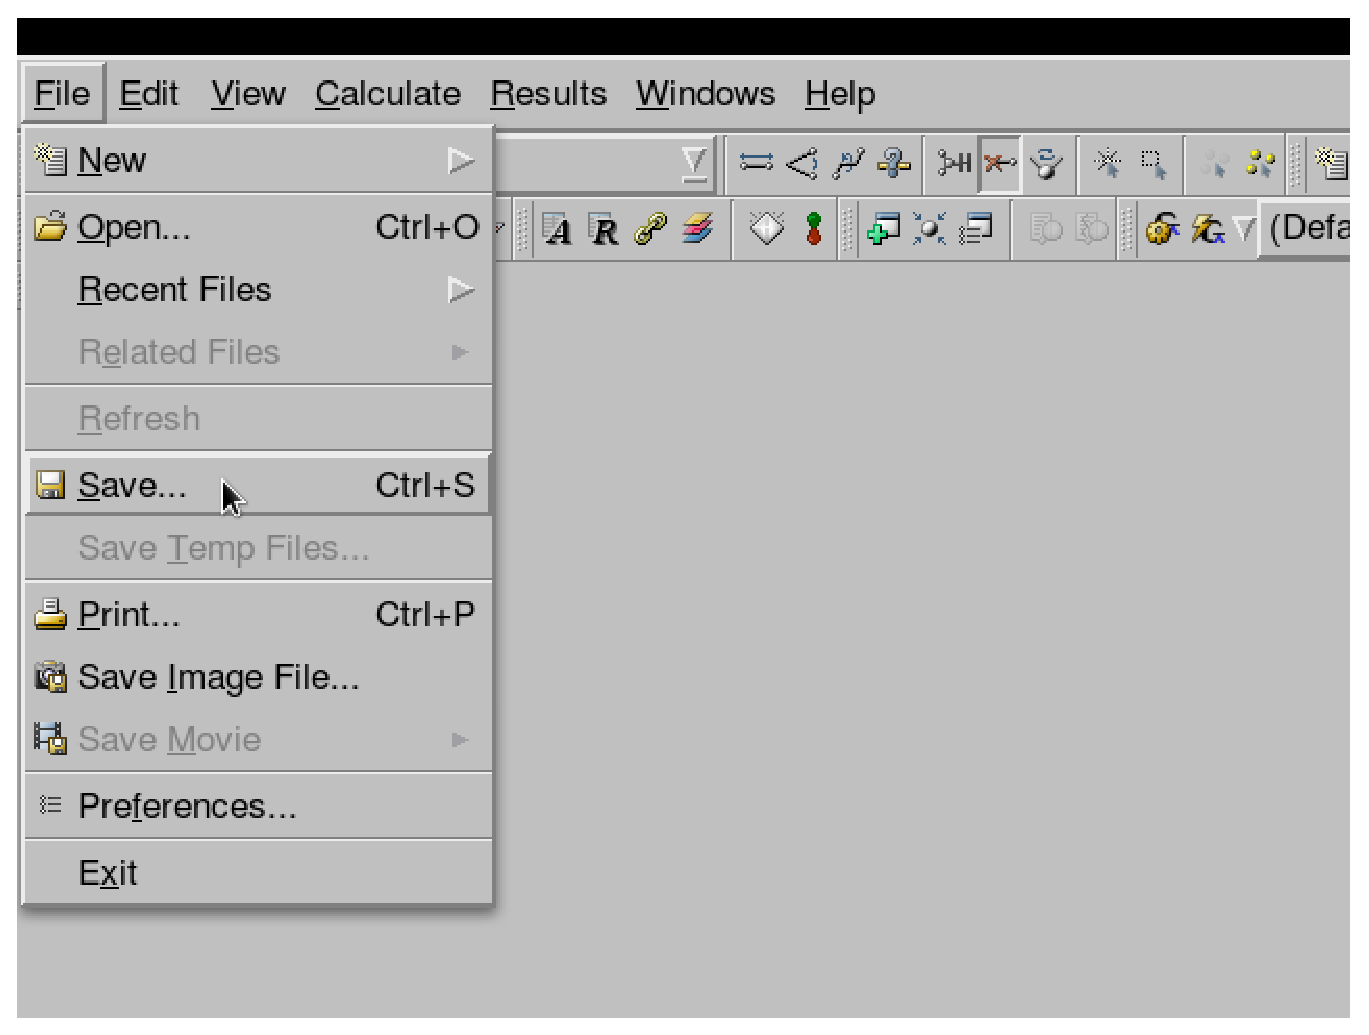
\includegraphics[height=2.5in]{gaussian8final.eps}
%\end{center}
%\end{figure}
%
%Type the name of the file and select PDB as the file type from the bottom menu.
%
%\begin{figure}[h]
%\begin{center}
%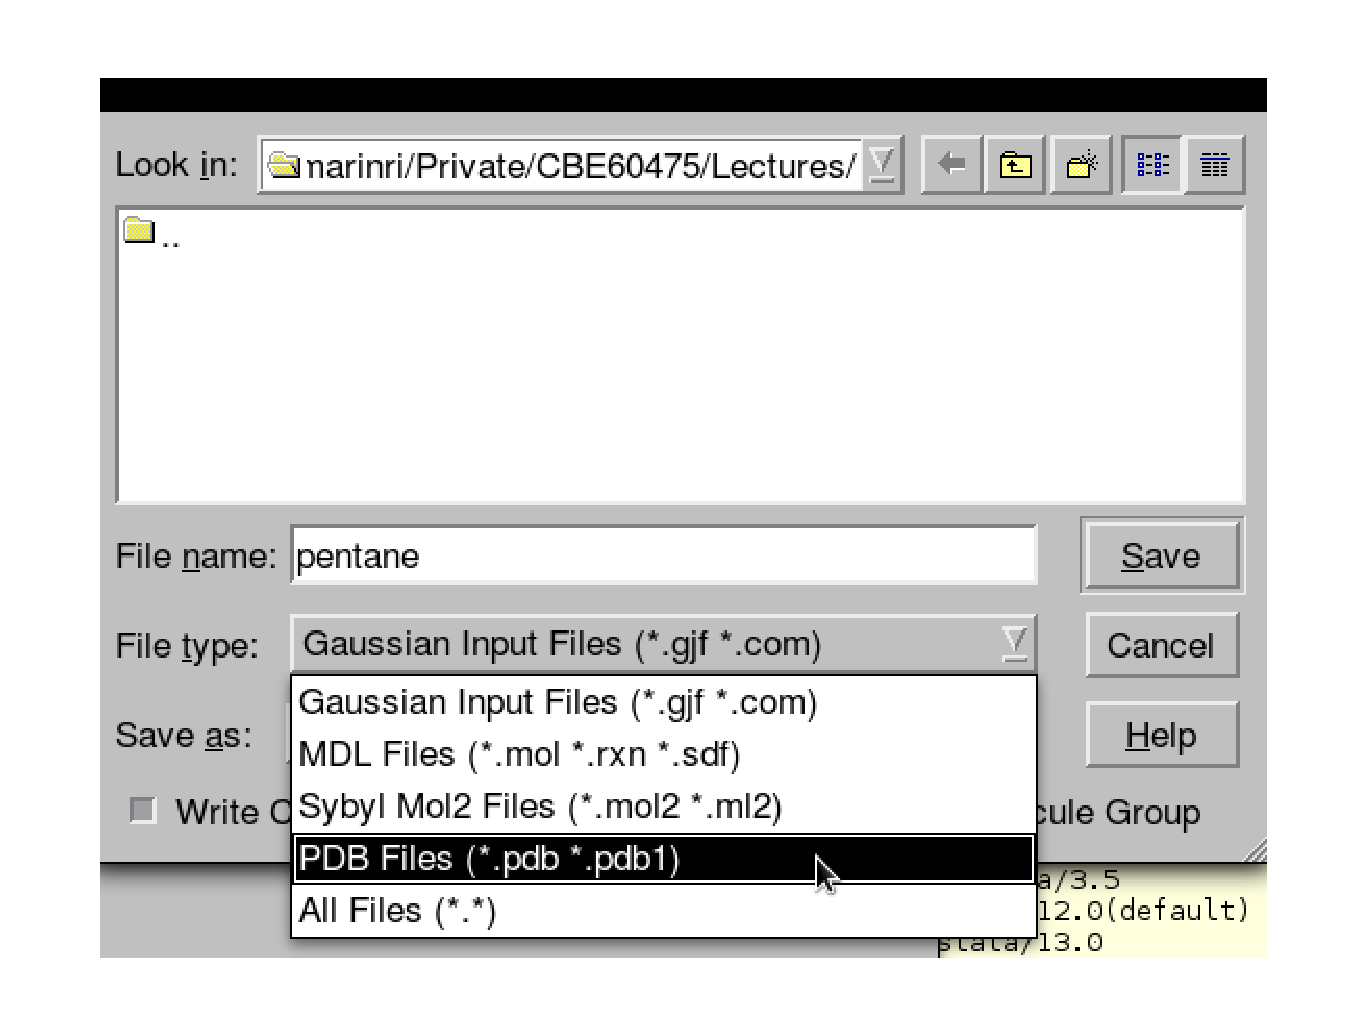
\includegraphics[height=2.5in]{gaussian9final.eps}
%\end{center}
%\end{figure}
%
%\vspace{3in}
%Close Gaussview. Back in the terminal, open the PDB file using your favorite text editor.

\begin{figure}[h]
\begin{center}
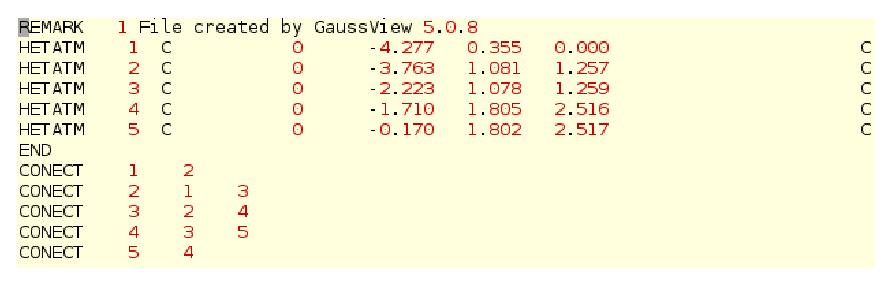
\includegraphics[height=1in]{pdbfile_final.eps}
\end{center}
\end{figure}

Append a column containing the atom types.

\begin{figure}[h]
\begin{center}
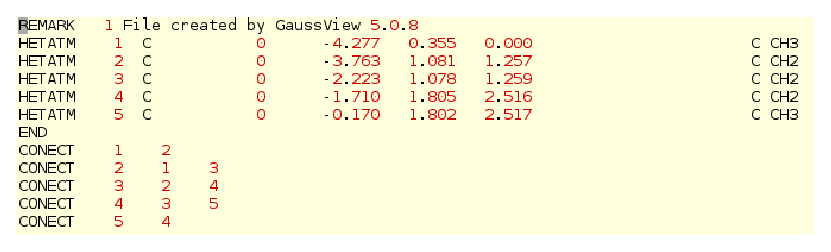
\includegraphics[height=1in]{pdbfile_edited_final.eps}
\end{center}
\end{figure}

Avogadro v1.1.1 can also be used to generate CML files. Below is an example of a 
CML file generated using Avogadro

\begin{figure}[h]
\begin{center}
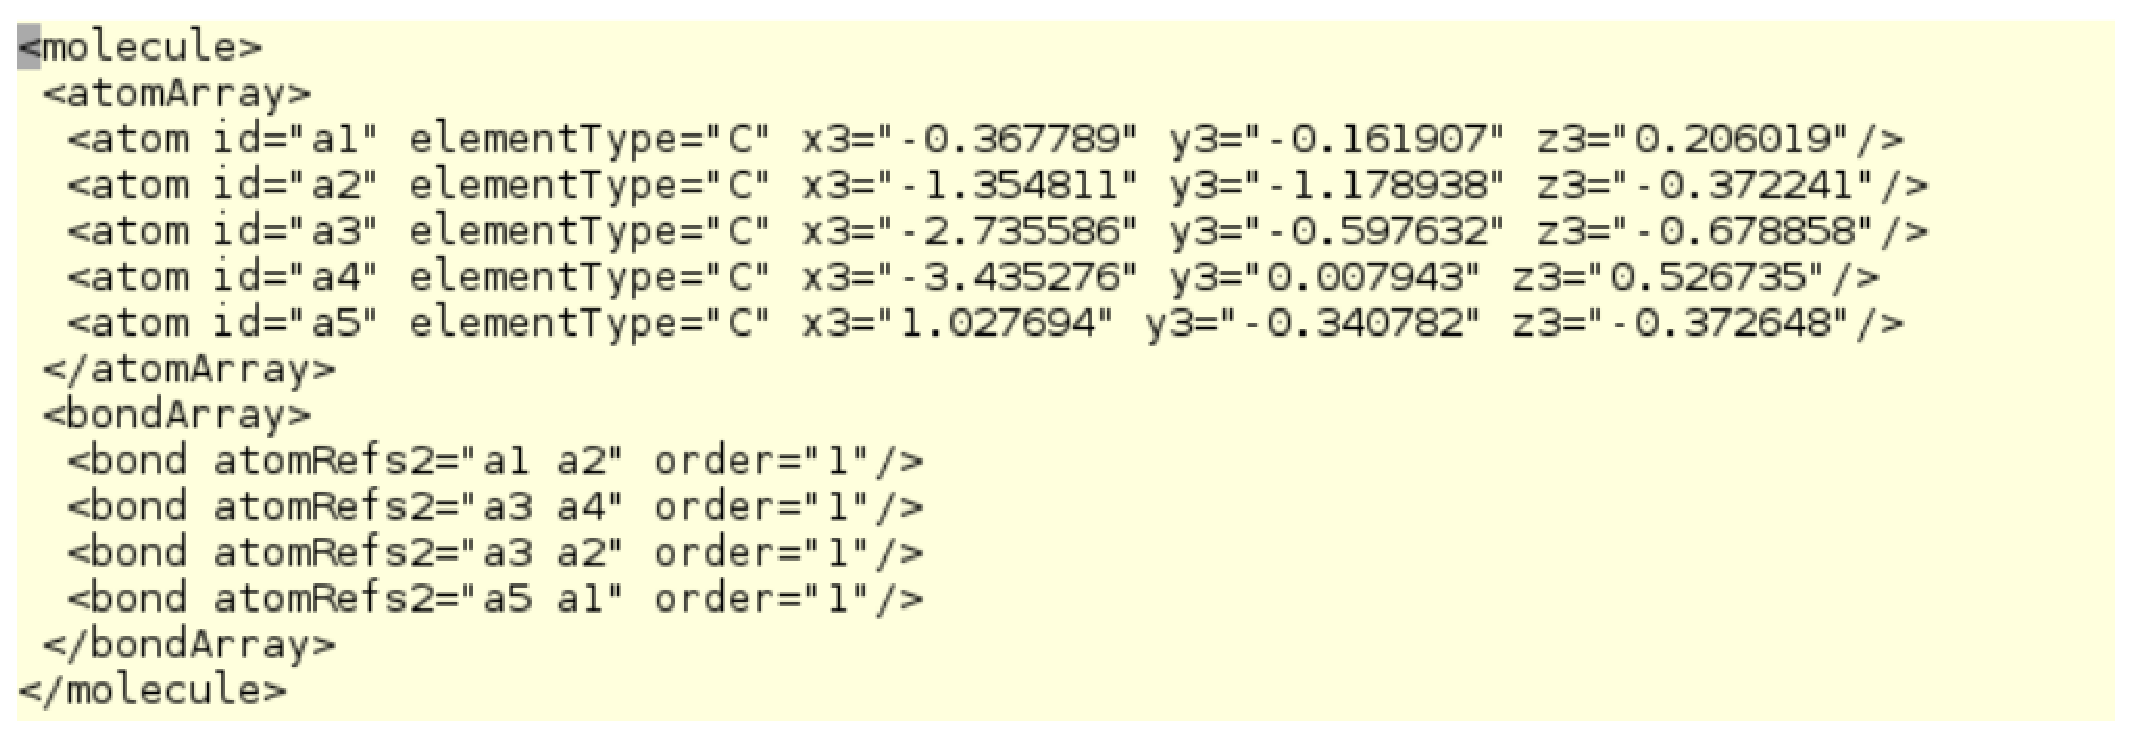
\includegraphics[height=1.5in]{pentane_cml.eps}
\end{center}
\end{figure}

\vspace{3in}
Modify the pentane united atom CML file. Note that the atom type is appended as a last
column between quotation marks.

\begin{figure}[h]
\begin{center}
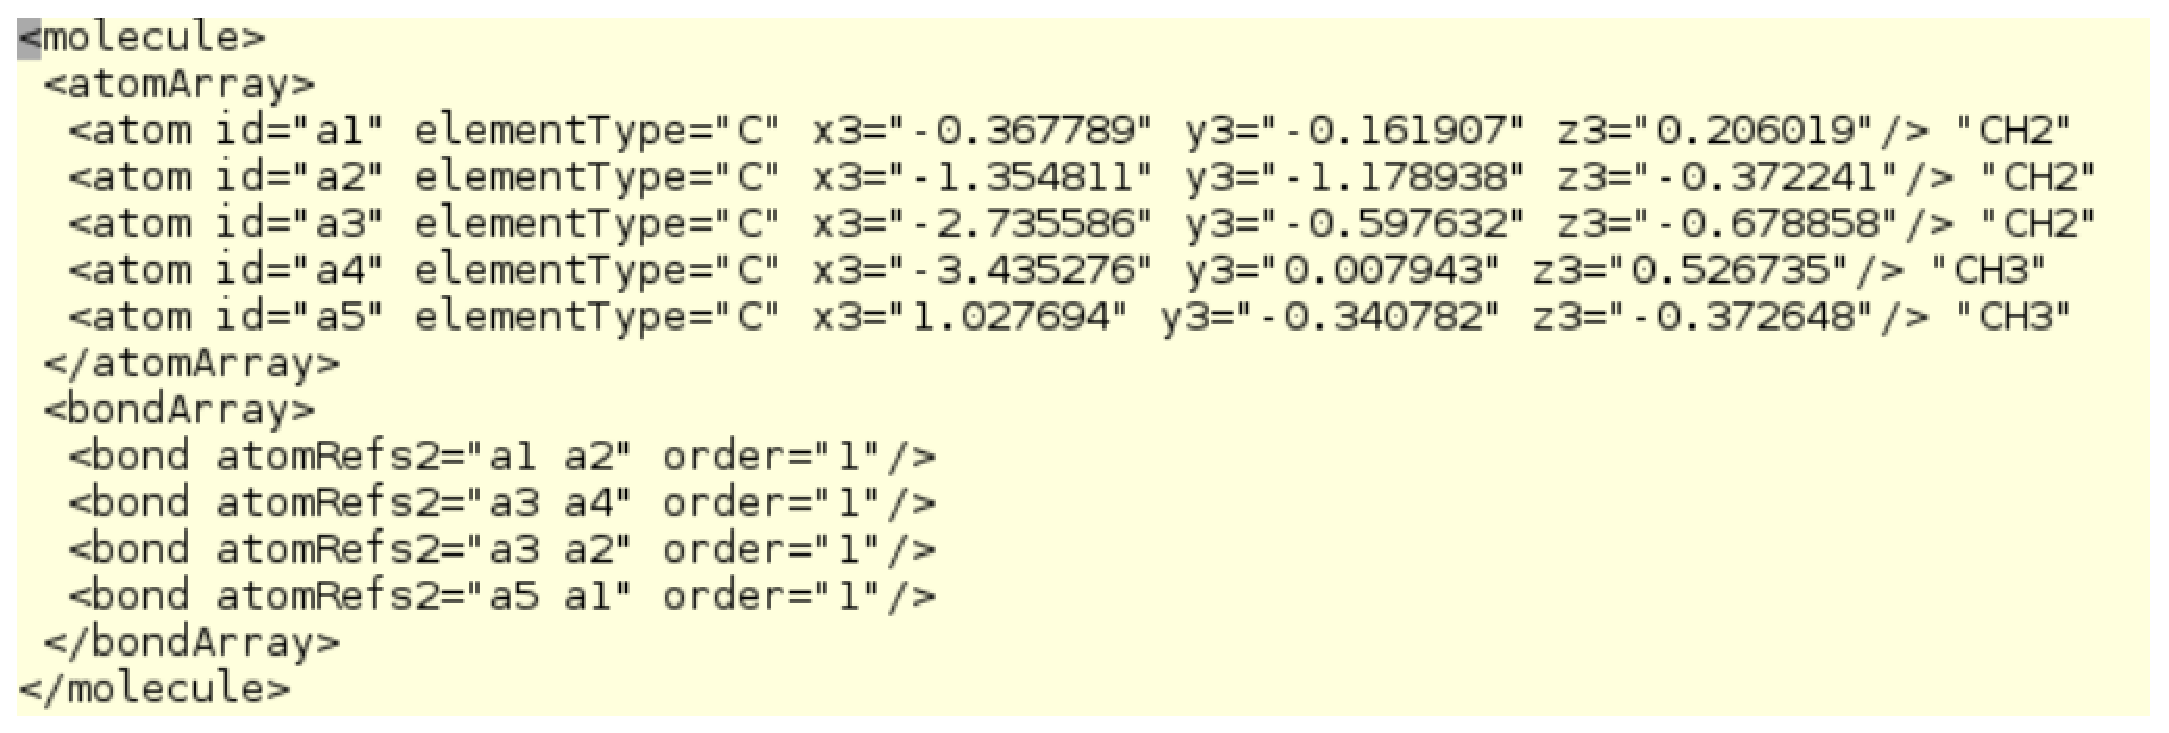
\includegraphics[height=1.5in]{pentane_cml_modified.eps}
\end{center}
\end{figure}

In the terminal, run the following command:\\ \\
\texttt{>python mcfgen.py pentane.pdb --ffTemplate}

This command will create an .ff file. The first three sections of the FF file are displayed next. 
Do not modify these.

\begin{figure}[h]
\begin{center}
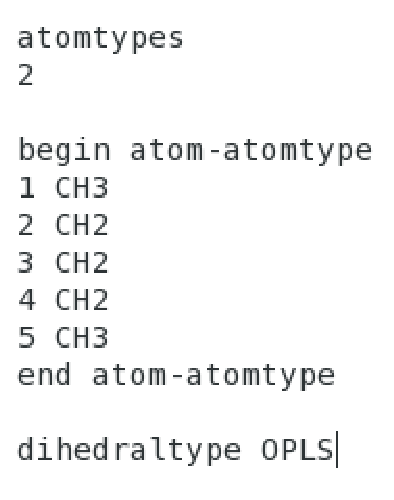
\includegraphics[height=2in]{top_ff.eps}
\end{center}
\end{figure}

The force field parameters for non-bonded (not shown), bonded, angle, dihedral (not shown)
and coulombic interactions (not shown) must be entered next to the corresponding keyword.
For example, the angle type CH3 CH2 CH2 has an angle of 114.0. This value must be placed
next to the ``Angle'' keyword.

\begin{figure}[h]
\begin{center}
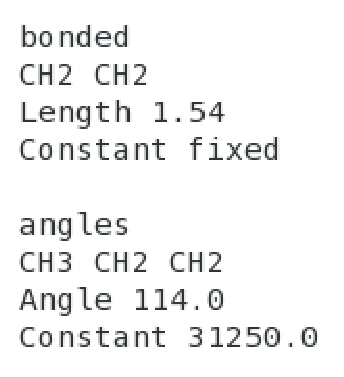
\includegraphics[height=1.5in]{body_ff.eps}
\end{center}
\end{figure}

\vspace{3in}
For more examples of filled ff files, please refer to the examples contained in the /Scripts/MCF\_Generation/ directory. Using the
filled .ff file, run: \\

\texttt{> python mcfgen.py pentane.pdb} \\

Check the file newly created pentane.mcf for any possible errors. This example can be found in the directory 
/Scripts/MCF\_Generation/PDB/

Note that if an MCF for a rigid solid is being created, this last step must include the --solid flag, as

\texttt{> python mcfgen.py zeolite.pdb --solid} \\

\section{Generate Library of Fragment Configurations}
\label{sec:libgen}

The goal of the script \texttt{library\_setup.py} is to automate the generation of fragment libraries.
As a starting point, the script requires the simulation input file, and the MCF and PDB 
files for each of the species. To run this script, type \\

\texttt{> library\_setup.py \$PATH\$/cassandra.exe input\_file.inp pdbfilespecies1.pdb pdfilespecies2.pdb ...} \\

This script will create the necessary files to create the fragment libraries. It will also run Cassandra 
to generate these libraries, whose location will be at \\

\texttt{/species?/frag?/frag?.inp} \\

where '?' refers to the species number, for example, species 1, species 2 etc. \\

Note that the script overwrites the section of the input file where 
needed (i.e. \# Frag\_Info) with the aforementioned directory locations.
